\chapter{The Low-Rate Regime and the Exclusion Bound}\label{ch:lowrate}

\needswork{STATUS: DRAFTED. This chapter carries the thesis's most durable result and also its
most uncomfortable self-correction. Both are stated here rather than in a limitations section.}

\section{Why the low-rate arm is a different regime, not a slower one}

The 802.11 numbers do not transfer. They differ by two to three orders of magnitude, and the
binding constraint differs \emph{in kind}: a regulatory airtime quota rather than a frame size or a
latency budget. This is the third regime in the taxonomy of \Cref{thm:t2a}:

\begin{center}
\begin{tabular}{lll}
\toprule
regime & what caps the batch & where \\
\midrule
MTU-limited & frame size & --- \\
freshness-limited & $\Lambda_i \Dmax$ & \textbf{802.11} \\
\textbf{duty-cycle-limited} & regulatory airtime quota & \textbf{low-rate} \\
\bottomrule
\end{tabular}
\end{center}

On this arm the arrival rate and the freshness are \emph{derived}, not configured: a frame of
airtime $T$ may repeat only every $T/\text{duty}$, so the sustainable rate and the staleness of the
oldest record are the same interval. There is no independent deadline to trade against bytes.

\section{The exclusion, and what part of it is arithmetic}

Applying \Cref{thm:t6} to EU868, with $\Hf = 44$\,B measured, $\ga = 64$\,B and $\smin = 13$\,B:

\begin{table}[h]
\centering
\caption{The EU868 partition. \textbf{Read the tier column, not just the verdict}: it says what
would have to change.}
\label{tab:t6}
\begin{tabular}{llrll}
\toprule
DR & payload $M$ & $\smax$ & tier & durability \\
\midrule
0, 1, 2 & 51\,B  & $-57$ & \textbf{signature} & \textbf{unconditional} \\
3       & 115\,B & $7$   & encoding & contingent --- see below \\
4, 5, 6 & 242\,B & $134$ & ---      & feasible \\
\bottomrule
\end{tabular}
\end{table}

\begin{figure}[h]
\centering
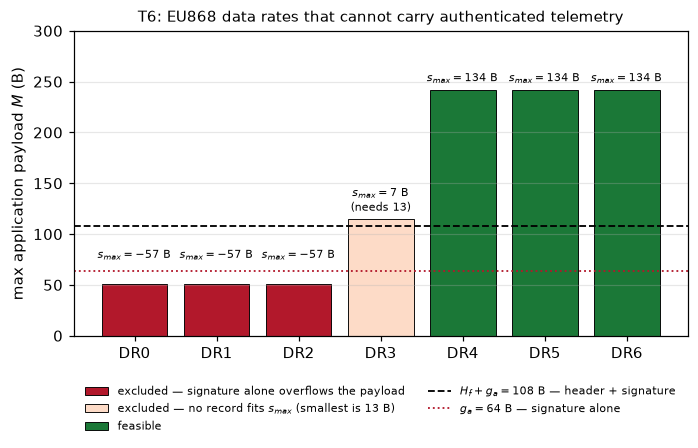
\includegraphics[width=0.75\textwidth]{fig_t6_exclusion.png}
\caption{Exclusion tiers across EU868 data rates.}
\label{fig:t6}
\end{figure}

\subsection{The three rates that cannot be rescued}

DR0--DR2 stay excluded \emph{with a zero-byte header and a one-byte record}. It is the signature
alone that does not fit: $64 > 51$. No header design, no encoding, no batching and no chain
placement reaches them. The only escape is a smaller authentication object, and the smallest
standardised one at comparable security is a $48$\,B compressed BLS12-381 G1 point --- which does
fit $51$\,B, and leaves \emph{three bytes} for the header and the record together.

\textbf{This is arithmetic. It does not move as hardware, models or schemes improve.} It is the
thesis's most durable claim and the reason the work is framed as a boundary.

\subsection{The fourth rate, which this thesis excluded by its own framing}

DR3 misses by six bytes. That margin rests on three constants, and \textbf{each of them is ours}:

\begin{enumerate}
\item $\Hf = 44$\,B, which is the \emph{top} of a measured $38$--$44$\,B range
      (\Cref{tab:hf}), and larger headers make exclusion more likely.
\item The payload column: published EU868 tables differ, and one source lists DR3 at $123$\,B where
      this work uses $115$\,B. At $123$\,B the residual is $15$\,B and \textbf{DR3 is feasible}.
\item $\smin = 13$\,B, the smallest record \emph{this design} can emit.
\end{enumerate}

\begin{remark}[The self-correction, stated plainly]
The frame header is $29$\,B of CBOR \emph{text key names}. The same seven keys encoded as small
integers cost $7$\,B --- the convention COSE and SenML already use. That single change takes
$\Hf$ from $44$ to $22$\,B, DR3's budget from $7$\,B to $29$\,B, and \textbf{makes DR3 feasible}.

The system-model chapter had always recorded that the header was untuned. The theory chapter had
always recorded that the bound depends on the header. \emph{Nobody put the two facts side by side.}
When they were, the headline moved from \textbf{four} excluded data rates to \textbf{three}.

Not even the record-field elision is required; halving the header suffices.
\end{remark}

\subsection{Why the smaller result is the better one}

Reporting three rather than four costs a memorable number and buys three things.

It is \emph{honest}: the four-rate claim was one reviewer's wire-format question away from being
wrong, and that reviewer would have been right. It is \emph{durable}: what remains cannot be
attacked by any framing work. And it makes the boundary \textbf{constructive} --- it says not only
where authentication cannot fit, but exactly what would have to change, and shows that for DR3 the
answer is a header redesign rather than new cryptography.

The tier taxonomy of \Cref{thm:t6} always named ``encoding'' as the tier compression can attack.
This is that tier being attacked, and moving, exactly as the taxonomy predicted.

\section{Per-frame chaining, and why the arms differ}

Moving the chain hash from per-record to per-frame is worth far more here than on 802.11, because
the regional payload limit binds --- so smaller records convert into \emph{more records per frame},
which the duty cycle turns directly into sustainable rate. Measured across DR4--DR6 it gives
$\approx 3.0\times$ the sustainable telemetry rate for the same regulatory budget.

\begin{figure}[h]
\centering

\includegraphics[width=0.7\textwidth]{fig_lora_chain.png}
\caption{Per-frame versus per-record chaining across data rates.}
\label{fig:lorachain}
\end{figure}

The 802.11 arm keeps per-record chaining, because freshness binds there and the same change buys
almost nothing in extra records --- too little to pay for losing independently-transmitted
per-record tamper evidence. \textbf{The two arms carry the same ledger in two framings, and that
asymmetry is the point rather than an inconsistency.}

\section{Capacity, and a threshold applied to the wrong thing}

Everything else in this arm is analytical and deliberately so --- time on air is a specification
formula and the sustainable rate is the duty cycle, both deterministic, so simulating them would be
circular. Exactly one quantity resists that: \emph{how many nodes can share the channel}, because
uplinks are pure ALOHA with no carrier sense.

Simulation at DR5 gives $\Nmax = 3$ against the $V \geq 0.95$ criterion.

\begin{remark}[Never quote this bare]
The bootstrap interval is $[2, 3]$ --- a knife edge --- and at the certified $N = 3$, \textbf{nine of
thirty seeds fail the very criterion being certified}. Under a per-realisation reading, where at
least $95\%$ of runs must individually meet $V$, the answer is \textbf{1}, not 3.

Both are computed and emitted. The decision to headline the mean is recorded as a decision, and it
was safe to take only because the comparative result survives either reading.
\end{remark}

An earlier value of $\Nmax = 5$ came from a three-seed sample against a bimodal distribution and is
retracted; the artifact that produced it is retained, renamed and superseded.

\subsection{External corroboration, quoted as a curve}

An external hardware-grounded model gives $\Nmax = 4$ where this work gives $3$.

\begin{remark}[Two cautions about that comparison]
Their $\Nmax$ is decided at $N = 4$ and $N = 5$, both inside the region their own fit is
intercept-dominated: the polynomial predicts $1.78\%$ loss at \emph{zero} transmitters, roughly
$40\%$ of the entire loss budget the criterion allows. Forcing the fit through the origin would give
them $\Nmax = 5$, \emph{widening} the gap --- so quoting $4$ is the conservative choice.

And the pessimism ratio is not a single number. It runs $0.91\times$ at $N = 2$, where \emph{this
work is the more optimistic model}, through $1.07\times$ at $N = 3$, to $2.1\times$ from $N = 10$
upward. The sign changes in exactly the region where $\Nmax$ is decided. An earlier finding in this
project quoted a single ratio in the wrong direction and had to be retracted.
\end{remark}

\section{Scope of this chapter}

This is simulation and analysis, not measurement. No radio was metered, and there is no energy
column --- the only measured radio power in this project is a Wi-Fi figure, and reusing it for a
different transceiver would be fabrication. Airtime per record is reported instead: it is what the
regulator rations, and it is computed rather than assumed.
